\chapter{Experiments}
As we have covered, the effect of a Multi-Task problem setting is challenging to quantify theoretically without experiments.
Here we will take various datasets for object recognition, object detection, and pose estimation and see what the effects of training them in a Multi-Task setting are.
The metrics we are mainly interested in are the reduction in model size, inference time, and model accuracy on the different tasks compared to the single-task counterparts.
We will also attempt to find out how much more difficult the training process and tuning various hyperparameters are when compared to the single-task problem.
The main focus will be on trying out the EfficientNet architecture as a backbone, but we will compare it to an equivalent ResNet model in some cases.

\section{Training setup}
All the experiments use the same computer, and the model training is done using an Nvidia GeForce RTX 2070 GPU that has 8 GB of GDDR6 VRAM \citep{nvidiaRTX}.
Thus all the models will have to be small enough to train on this relatively small amount of memory.
The deep learning framework that is used to implement the models in all the experiments will be PyTorch \citep{pytorch} that is used inside Docker \citep{docker} containers.
Also, Nvidia Apex \citep{Apex} will be used to train models using mixed precision floating-point numbers to reduce the size of the models and to increase the speed of floating-point operations.
The model weights will be 16-bit floating-point numbers where it is safe to use the lower precision representation.
Besides the performance improvement, using lower precision floating-points can act as a regularizer as the model can't overfit on the high precision values and thus improve model accuracy as well \citep{mixedTraining}.

As a default for each task, we will use the following default procedures unless otherwise stated.
For the Multi-task training process, we will sample the data sets for each task with a probability respective to its size.
The loss function for every task has the same weight multiplier of one.
The batch size for each task will be maximized to fit within the memory requirement, giving a batch size of 32.
For weight optimizer, we will use SGD with a cyclic learning rate scheduler \citep{cycliclr}.


\section{Multiple object classification tasks}
As we have previously covered, fine-tuning an ImageNet classifier often produces good results.
Here we will take a pre-trained EfficientNet backbone and learn multiple object classification tasks using the shared image embedding.
First, we will use two datasets that both contain images of healthy and unhealthy plants.

The ibean dataset \citep{beansdata} contains 1296 images classified into three classes; Healthy, Angular Leaf Spot, and Bean Rust.
The citrus leaves dataset \citep{citrusdata}, on the other hand, contains 594 examples of citrus fruits and leaves with four different classes; Black Spot, Canker, Greening, and Healthy.
Both of these datasets have a relatively small amount of images available for training, and training on only one of them could easily lead the model to overfit or not generalize well.
When the two closely related datasets are used to train the model, we could expect the model to generalize better on both of them, as hopefully similar features would benefit both tasks.
This model is depicted in figure 7.1.

\begin{figure}[h!]
    \centering
    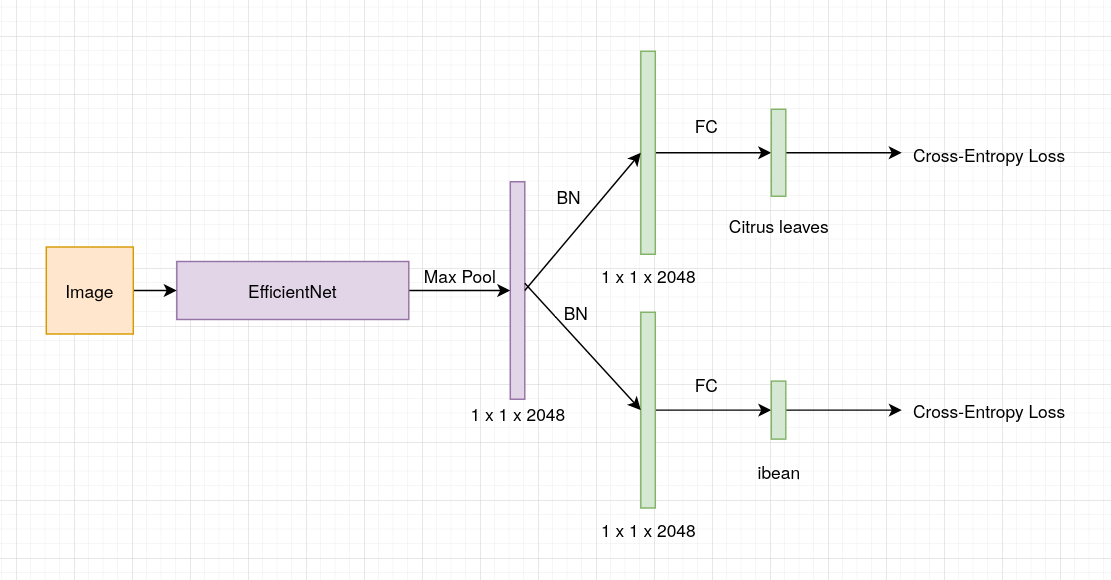
\includegraphics[width=0.8\textwidth]{imgs/object_classification_architecture.png}
    \caption{Network architecture for two image classification tasks.}
\end{figure}

To further extend the generalizability, we will try to add a third somewhat similar classification task using the TensorFlow flowers dataset \citep{tfflowers}, which contains five different types of flowers.
The assumption here would be that flowers could require similar features as the previous leaf classification tasks, thus when increasing the training data with a closely related task, we could increase the generalizability even further.

\section{Different tasks using shared representation}
Here we will create similar models to \citep{visualPerson}, but using EfficientNet, and then we will add a shared object detector to detect the people.

\section{Multiple object detectors}
Train multiple object detector using shared representations